\section{Overview of Traffic Simulators}

    \frame{\sectionpage}
    
    \begin{frame}{What is a Traffic Simulator?}
        \begin{itemize}
            \item \textbf{Network}: infrastructure (real, virtual, etc) that allow the flow of objects or information
            \item \textbf{Traffic}: objects (or packets) that transverse the network
            \item \textbf{Simulation}:  modeling the flow of traffic on the network over time
            \vspace{22pt}
                \item Macroscopic:  models flow and patterns
                \item Microscopic:  models individual units
        \end{itemize}
    \end{frame}    
    
    \begin{frame}{Existing Simulations}
        \begin{figure}
            \centering
            \begin{figure}[ht]
                \begin{minipage}[b]{0.45\linewidth}
                    \centering
                    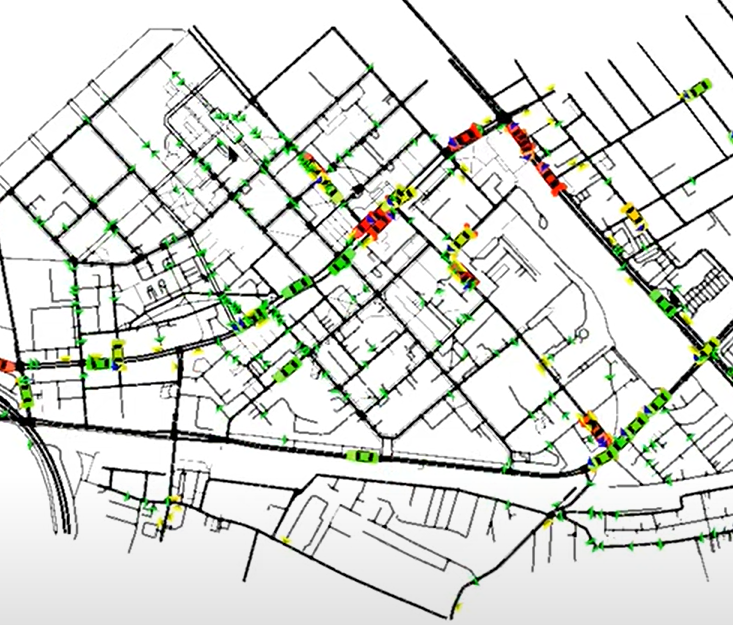
\includegraphics[width=\textwidth, height=5cm]{Images/sumo_ex_cropped.png}
                    \caption{SUMO \cite{SUMO2022}}
                    \label{fig:a}
                \end{minipage}
                \hspace{0.5cm}
                \begin{minipage}[b]{0.45\linewidth}
                    \centering
                    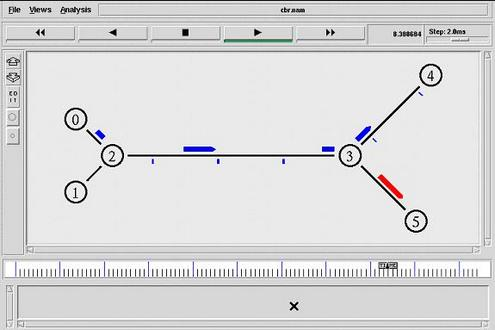
\includegraphics[width=\textwidth, height=5cm]{Images/NS2-simulator.jpg}
                    \caption{NS2 \cite{absingh}}
                    \label{fig:b}
                \end{minipage}
            \end{figure}
        \end{figure}
    \end{frame}
    

   